% IEEE two-column manuscript based on the official IEEE LaTeX package
% downloaded from the IEEE Template Selector on 2026-10-05.
\documentclass[10pt,journal,a4paper]{IEEEtran}

\usepackage{cite}
\usepackage{amsmath,amssymb,amsfonts}
\usepackage{graphicx}
\usepackage{textcomp}
\usepackage{xcolor}
\usepackage{url}
\usepackage{orcidlink}
\usepackage{booktabs}
\usepackage{tikz}
\usetikzlibrary{arrows.meta}
% Keep the framework and VGC mechanism on separate double-column float tops.
\setcounter{dbltopnumber}{1}
% Keep draft notices visible until measurements and their provenance are verified.
\newif\ifdraftpaper
\draftpapertrue
\newcommand{\draftnote}[1]{\ifdraftpaper\par\smallskip\noindent\textit{Draft status: #1}\par\smallskip\fi}
\newcommand{\pending}{\textnormal{TBD}}
\hypersetup{
	colorlinks=true,
	linkcolor=blue,
	citecolor=blue,
	urlcolor=magenta,
	filecolor=magenta
}

\begin{document}

\title{Mind the Sky: Resolving Sky-Depth Collapse with Validity-Guided Diffusion}
% 考虑一下 sky-depth inconsistency ？这里我认为需要思考什么是塌陷，什么是不一致性的问题。 先放着。

\author{
    Jiawei~Wang\textsuperscript{\textdagger,*}\orcidlink{0009-0006-0793-6698},
    Jingxuan~Wang\textsuperscript{\textdagger}\orcidlink{0009-0002-9606-4748},
    Mingbo~Lei\orcidlink{0009-0001-3198-8045},
    Liang~Yao,
    Jiayi~Li, and Tianyu~Lu%
    \thanks{Jiawei Wang, Mingbo Lei, Liang Yao, and Jiayi Li are with the School of Computer Science and Engineering, Shenyang Jianzhu University, Shenyang, China, and the National Special Computer Engineering Technology Research Center (Shenyang Branch), Shenyang, China.}%
    \thanks{Jingxuan Wang is with the School of Chinese Medicine, Beijing University of Chinese Medicine, Beijing, China.}%
    \thanks{\textdagger\ Jiawei Wang and Jingxuan Wang contributed equally to this work.}%
    \thanks{This work was conducted by Jiawei Wang during an internship at \textbf{Infiniflow (Shanghai) Information Technology Co., Ltd.}}%
    \thanks{* Corresponding author: Jiawei Wang (e-mail: Haruko386@outlook.com).}%
}
\IEEEaftertitletext{%
    \vspace{-3.5em}
    \begin{center}
        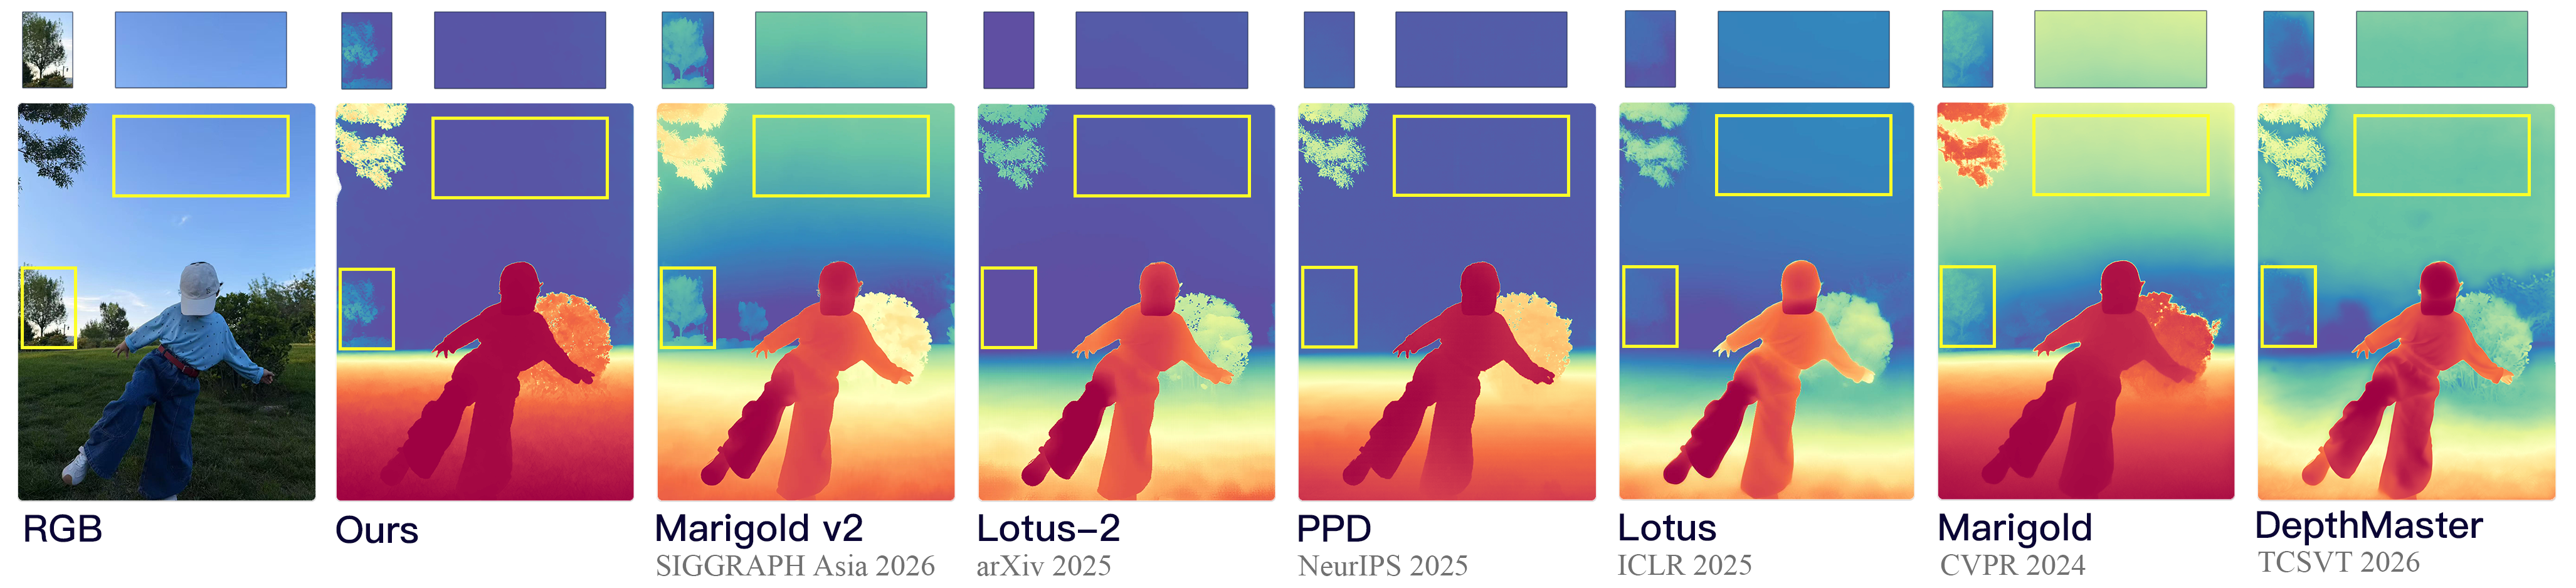
\includegraphics[width=\textwidth]{img/banner-hor.png}
    \end{center}
    \vspace{0.5em}
}

\maketitle

\begin{abstract}
	Diffusion-based monocular depth estimation can recover detailed scene geometry, yet their outdoor predictions may assign nearby depths or artificial depth variations to the sky.
	We study this sky-depth collapse as a supervision problem: depth validity masks remove unreliable measurements, but can also leave large sky and out-of-range regions without a direct training signal.
	We present ApDepth-G, a multi-step latent diffusion framework that addresses this gap through validity-guided completion. The method separates fully valid, fully invalid, and mixed latent cells,
	applies weak region-level anchoring and interior smoothness on invalid support, and adds a selective far-field anchor to reduce the ambiguity of distant regions. We use a frozen depth estimation model as
	an auxiliary condition and a weak reference. To make the denoising trajectory consistent with its pure-noise initialization,
	we combine terminal-SNR alignment with a velocity objective and endpoint-aware noise augmentation. The resulting formulation is designed to improve sky stability while preserving supervised foreground
	structure, without requiring sky annotations during training. Code is available at \url{https://haruko386.github.io/ApDepth-G/}.
\end{abstract}

\begin{IEEEkeywords}
	Monocular depth estimation, sky-depth collapse, latent diffusion, validity-guided completion.
\end{IEEEkeywords}

\section{Introduction}
\label{sec:introduction}
Monocular depth estimation recovers scene geometry from a single image and supports applications in reconstruction, robotics, and autonomous driving. 
A good depth map must represent both visible objects and their spatial relationship to distant backgrounds. 
This remains difficult because appearance does not uniquely determine geometry: a change in illumination or texture need not indicate a change in distance. 
Recent discriminative foundation models and diffusion-based models have substantially improved cross-domain prediction~\cite{Li2024DepthV2,Ke2025Marigold}, 
but ambiguous outdoor regions remain a practical source of error.

Pretrained image diffusion models offer rich visual representations that can be adapted to depth prediction 
using relatively limited geometric supervision~\cite{rombach2022high,ke2024repurposing}. Marigold demonstrates this transfer 
from image generation to dense image analysis~\cite{Ke2025Marigold,ke2024repurposing}. More recently, Marigold V2~\cite{pavlovic2026marigoldv2} studies the remaining reconstruction artifacts of 
adapted generative models and develops targeted representation and decoder refinement objectives~\cite{pavlovic2026marigoldv2}. 
These advances suggest that improving depth estimation requires understanding the particular failure of the adapted predictor, beyond increasing backbone capacity alone.

\begin{figure}[!t]
	\centering
	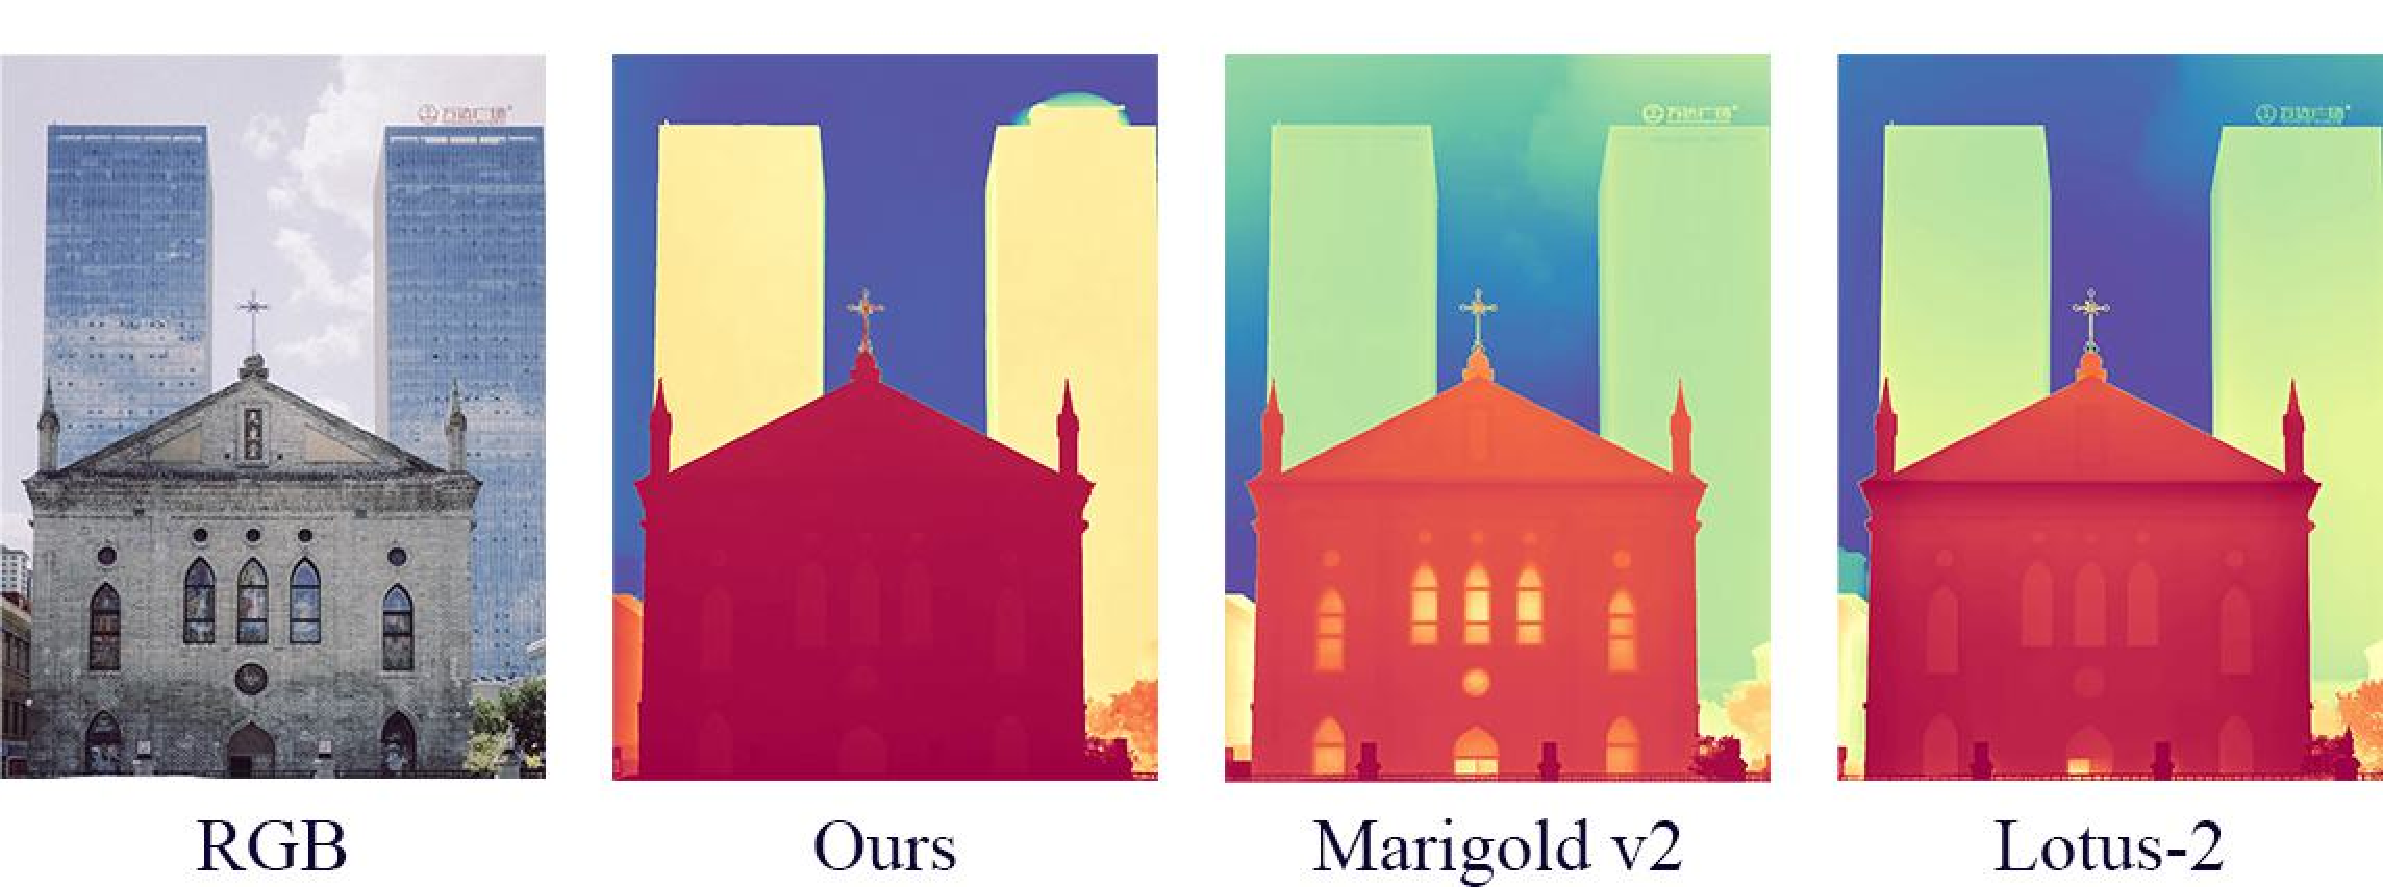
\includegraphics[width=\linewidth]{pdf/sky-collapse-multi-method.pdf}
	\caption{Comparison of sky-depth estimation across different diffusion-based methods. Existing methods often suffer from sky-depth collapse,
	incorrectly assigning smaller depth values to distant sky regions, particularly around clouds. In contrast, our method preserves spatially consistent
	far-depth predictions across the sky.}
	\label{fig:sky_depth_collapse}
	% \vspace{-1.8em}
\end{figure}

% 下面这一句的描述目前来看是有问题的，后面要改(哪里有问题了？光说不指出来？我先把这个注释留着，没准后面真有问题。后续改的时候顶多再注意一下，下次看如果还没啥问题就可删了)
Our focus is \emph{sky-depth collapse}. A model may delineate the sky correctly in appearance while assigning it 
depths comparable to nearby objects, or introduce gradients and cloud-shaped structures within the sky. 
In affine-invariant depth prediction, the desired behavior is not to output literal metric infinity. 
As illustrated in Fig.~\ref{fig:sky_depth_collapse}, sky should occupy a consistent far-depth range relative to the visible scene, without acquiring unsupported surface 
geometry. This distinction matters: identifying the sky boundary and assigning the correct depth ordering are different tasks.

A central difficulty lies in supervision coverage. 
Reliable depth is often unavailable for sky, while finite-range sensors and dataset validity thresholds 
exclude distant measurements. Masking these values is necessary, but the usual valid-pixel objective gives 
no direct target to the excluded region. Semantic knowledge from the image backbone does not 
by itself determine the numerical depth assigned there. Moreover, a low aggregate training loss can coexist with severe 
sky errors because those errors may lie outside the evaluated mask. We therefore treat the missing supervision as 
an explicit modeling issue, rather than assume that additional denoising steps will automatically correct it.

Depth invalidity also extends beyond sky. Figure~\ref{fig:invalid_region_img} shows a DIODE example in which both the sky and parts of a visible window lack valid depth observations. The validity mask therefore indicates supervision coverage rather than semantic sky membership.

\begin{figure}[!t]
	\centering
	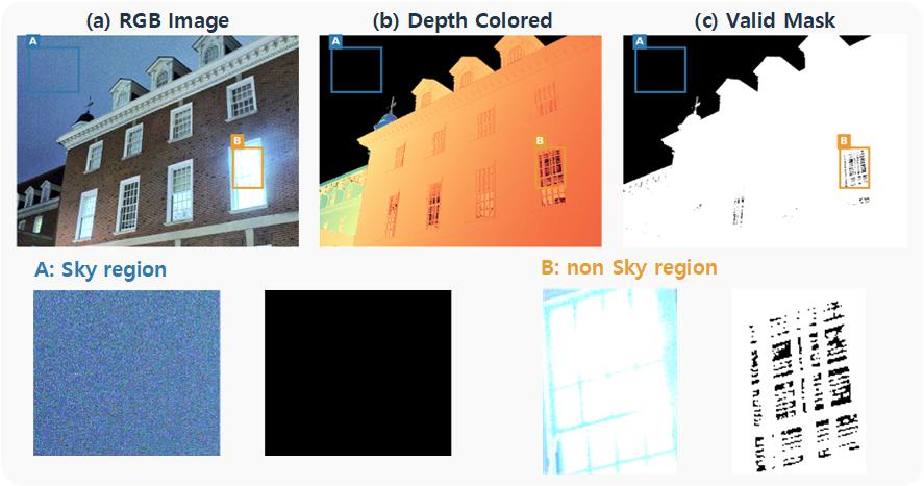
\includegraphics[width=\linewidth]{pdf/invalid_region_img.pdf}
	\caption{Depth invalidity beyond sky in a DIODE example~\cite{vasiljevic2019diode}. The top row shows (a) the RGB image, (b) the depth visualization, and (c) the dataset validity mask, where white denotes valid observations and black denotes invalid observations. The bottom row enlarges the RGB and mask crops marked A and B. Region A lies in the sky and has no valid depth; region B lies within a visible window and also contains missing observations. Thus, invalid depth does not uniquely identify sky.}
	\label{fig:invalid_region_img}
\end{figure}

We propose ApDepth-G, a multi-step diffusion fine-tune protocol centered on \emph{validity-guided completion} (VGC). 
Valid regions retain ordinary depth supervision. Large invalid regions receive weak, channel-wise regional anchoring and 
spatial regularization, while a selected far-field subset receives an additional regional anchor. 
All three constraints are defined in the depth latent space. They avoid copying a teacher's dense texture into 
every missing pixel and exclude finite differences across the valid/invalid boundary. Conservative masks and activation thresholds limit, but do not eliminate, the ambiguity of invalid-region selection.

ApDepth-G uses Depth Anything V2~\cite{Li2024DepthV2} as an auxiliary input and weak reference, 
following the prior-conditioned formulation of our earlier ApDepth model~\cite{wang2026apdepth}. 
This auxiliary estimate provides a semantic prior for depth prediction and a weak supervisory reference for sky regions lacking valid depth observations. 
The contribution is how incomplete supervision is handled within the diffusion objective. 
We further align the high-noise training endpoint with inference, adopting zero terminal signal-to-noise ratio (SNR), 
velocity prediction, and terminal-start sampling~\cite{lin2024common}. Structured noise augmentation is attenuated near 
this endpoint, and a small floor in the velocity-space Min-SNR weight retains supervision at pure noise. 
These choices address a separate source of train--inference mismatch while preserving multi-step denoising.

Our contributions are threefold:
\begin{itemize}
	\item We formulate sky-depth collapse as an underconstrained depth-assignment problem and distinguish sky consistency from accuracy measured only on valid foreground depths.
	\item We develop a validity-guided training objective with conservative latent masks, weak regional completion, and selective far-field anchoring to improve the stability of unsupervised distant regions.
	\item We incorporate validity-guided completion into a terminal-aligned multi-step diffusion framework, enabling the proposed completion objective to operate throughout the denoising trajectory while maintaining consistency between training and inference.
\end{itemize}

\section{Related Work}
\label{sec:related_work}
\subsection{Monocular Depth and Geometric Priors}
Learning-based monocular depth estimation has progressed from multi-scale CNN regression~\cite{eigen2014depth} to ordinal regression and 
adaptive-bin formulations~\cite{fu2018deep,bhat2021adabins}, and then to transformer-based dense prediction~\cite{ranftl2021vision}. 
Because metric depth is difficult to collect at scale and varies with camera parameters, another major line of work emphasizes relative 
or affine-invariant prediction and cross-domain transfer. MiDaS obtains robust relative depth by mixing heterogeneous datasets and resolving 
incompatible supervision~\cite{ranftl2020towards}; Depth Anything V2 combines large-scale pseudo-labeling with synthetic supervision to produce
 a strong general-purpose depth prior~\cite{Li2024DepthV2}; and MoGe jointly recovers monocular geometry for open-domain images~\cite{wang2024moge}. 
 These discriminative foundation models deliver strong global layout, but their success depends on large and diverse training corpora and does not eliminate 
 local ambiguity in invalid or weakly supervised regions.

BetterDepth provides the closest precedent for using such an estimate inside a diffusion depth model~\cite{zhang2024betterdepth}. 
It conditions an iterative refiner on the input image and a coarse prediction from a pretrained monocular estimator; global pre-alignment and local patch 
masking preserve the coarse global layout while diffusion recovers detail. ApDepth-G adopts this prior-conditioned formulation with Depth Anything V2-Giant, 
but targets missing outdoor depth, especially sky. Because the auxiliary disparity can have incompatible ordering and local errors, we correct its interface, 
retain measured depth wherever it is valid, and use the prior only as a bounded regional reference rather than dense ground truth.

\begin{figure*}[!t]
	\centering
	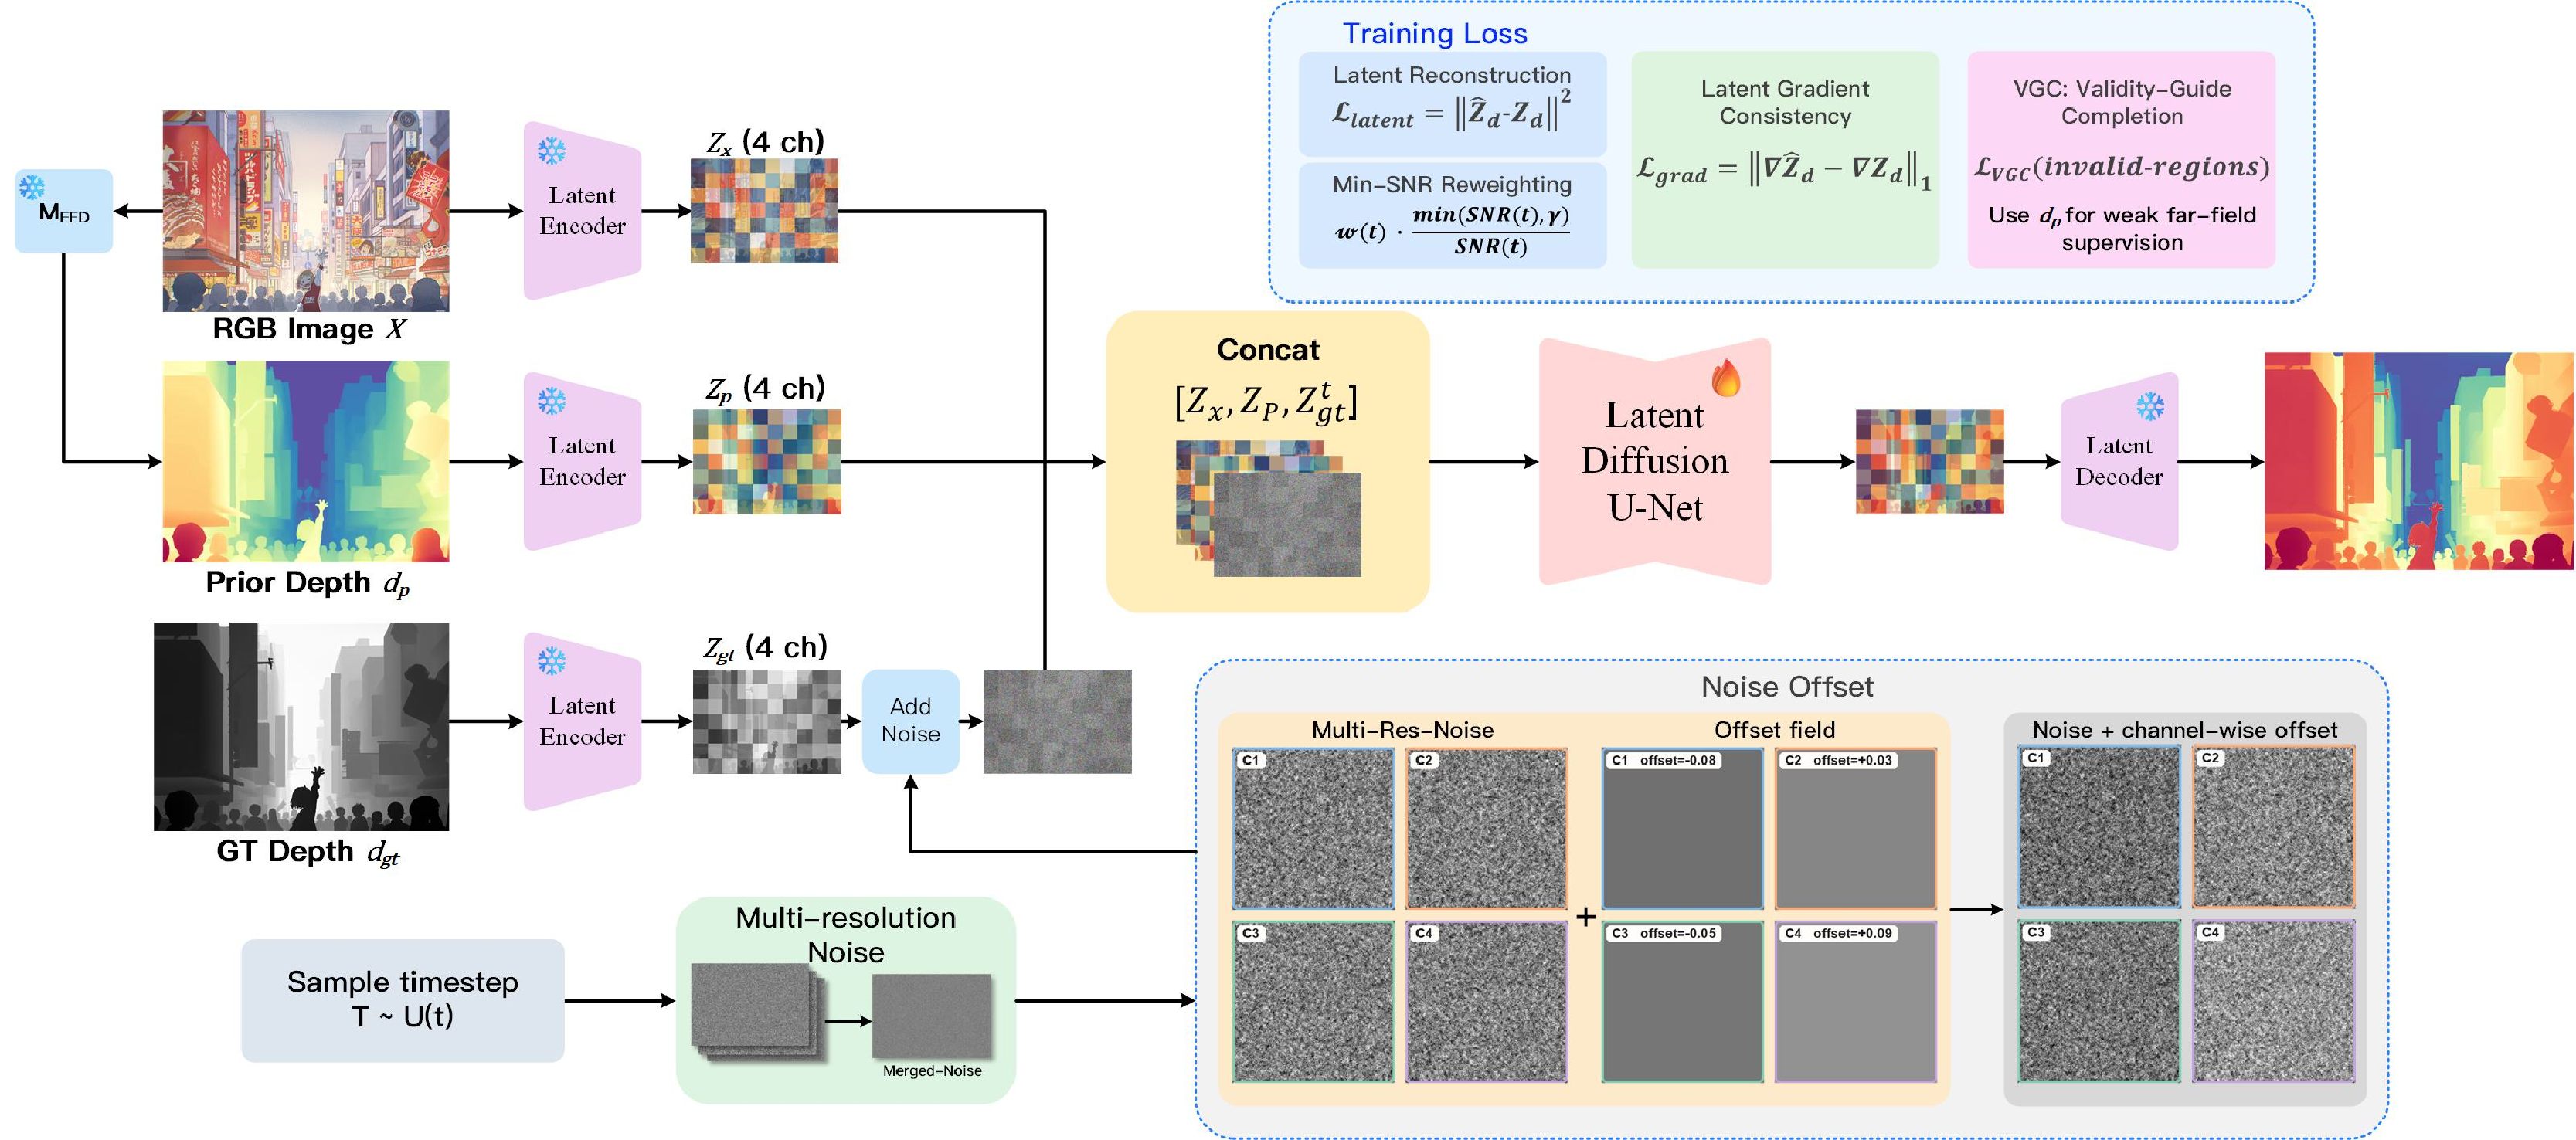
\includegraphics[width=\textwidth]{pdf/frame.pdf}
	\caption{Overview of ApDepth-G. A frozen depth estimator provides the auxiliary prior. The RGB, prior-depth, and noisy-depth latents form the twelve-channel input to the trainable U-Net, which predicts velocity. Training samples one timestep per image: the velocity error is supervised on fully valid cells, while gradient consistency and VGC act on the reconstructed clean latent $\hat z_0$ over their respective supports. The training objectives are defined in Secs.~\ref{sec:vgc} and~\ref{sec:diffusion}. At inference, noisy depth is initialized from a standard Gaussian and updated by 50 DDIM steps before decoding. Snowflakes and flames indicate frozen and trainable modules, respectively.}
	\label{fig:framework}
\end{figure*}

\subsection{Diffusion-Based Depth Estimation}
Early diffusion depth estimators learn a conditional denoising process directly over depth or disparity~\cite{saxena2023depthgen,duan2023diffusiondepth}.
 Marigold instead repurposes the visual prior of a pretrained latent image diffusion model using synthetic RGB--depth pairs, obtaining strong zero-shot 
 affine-invariant depth~\cite{ke2024repurposing,Ke2025Marigold}. This strategy established latent generative pretraining as a competitive alternative to 
 very large discriminative training sets. GeoWizard extends the idea to joint depth and surface-normal estimation~\cite{fu2025geowizard}, whereas DepthFM 
 formulates monocular depth through conditional flow matching to reduce sampling cost~\cite{gui2024depthfm}.

The iterative denoising inherited from image generation is expensive and stochastic, motivating deterministic or single-step adaptation. GenPercept analyzes the 
components required to transfer generative diffusion models to dense perception~\cite{xu2024genpercept}; E2E-FT revisits end-to-end fine-tuning and sampling choices~\cite{garcia2025fine};
 and Lotus tailors the diffusion formulation to dense prediction with single-step inference and detail preservation~\cite{he2025lotus}. DepthMaster further aligns generative features with 
 a semantic encoder and introduces Fourier enhancement in a two-stage training scheme~\cite{song2026depthmaster}. Lotus-2 combines a deterministic core predictor with constrained rectified-flow 
 refinement, targeting global consistency and sharper local geometry from only 59K training samples~\cite{he2025lotus2}. ApDepth likewise uses a pretrained depth condition in a single-step 
 formulation~\cite{wang2026apdepth}. These works demonstrate that fast inference need not discard the pretrained world prior, 
 but they also expose a recurring trade-off between global structure, boundary fidelity, and sampling cost.

Recent work places greater emphasis on high-resolution detail. Pixel-Perfect Depth (PPD) performs diffusion in pixel space to avoid VAE-induced boundary 
artifacts and uses semantic prompting plus a cascaded DiT design~\cite{xu2025pixel}. InfiniDepth represents depth as a neural implicit field that can be queried 
at arbitrary output coordinates~\cite{yu2026infinidepth}. FE2E starts from an image-editing DiT, whose structural conditioning is naturally compatible with image-to-image 
geometry prediction, and adapts its flow-matching objective for deterministic depth and normal estimation~\cite{wang2026fe2e}. Marigold V2 returns to a VAE-based DiT and uses 
representation alignment followed by Sinkhorn-based refinement to improve both geometry and fine structures~\cite{pavlovic2026marigoldv2}. 
These methods substantially sharpen visible boundaries; however, detail fidelity and numerical depth assignment are not identical.
 A visually coherent sky may still receive an incorrect relative depth when the corresponding pixels lack sensor supervision.

\subsection{Supervision and Diffusion Optimization} % 我这里也许需要去看一看这个SNR的论文了，不然不好给老登讲清楚
Diffusion fine-tuning is also sensitive to the distribution of timesteps and to the parameterization of the denoising target. 
Min-SNR weighting balances objectives whose gradient magnitudes differ across noise levels~\cite{hang2023efficient}. 
Lin et al.~\cite{lin2024common} identify a mismatch between common training schedules and inference that begins from pure noise, 
motivating zero-terminal-SNR schedules, velocity prediction, and sampling from the terminal timestep. We adopt these established optimization 
tools and combine them with endpoint-aware structured noise.

Our supervision problem is orthogonal to schedule correction. Commodity depth sensors frequently provide no valid target for sky, 
reflective surfaces, or out-of-range regions, so the usual reconstruction loss contributes no gradient there. 
Treating every invalid pixel as sky is unsafe, while copying a dense teacher everywhere would transfer its errors and undermine measured supervision. 
The proposed Validity-Guided Completion (VGC) therefore uses the auxiliary depth prior to provide weak, region-level supervision where valid depth observations are unavailable.

\begin{figure*}[!t]
	\centering
	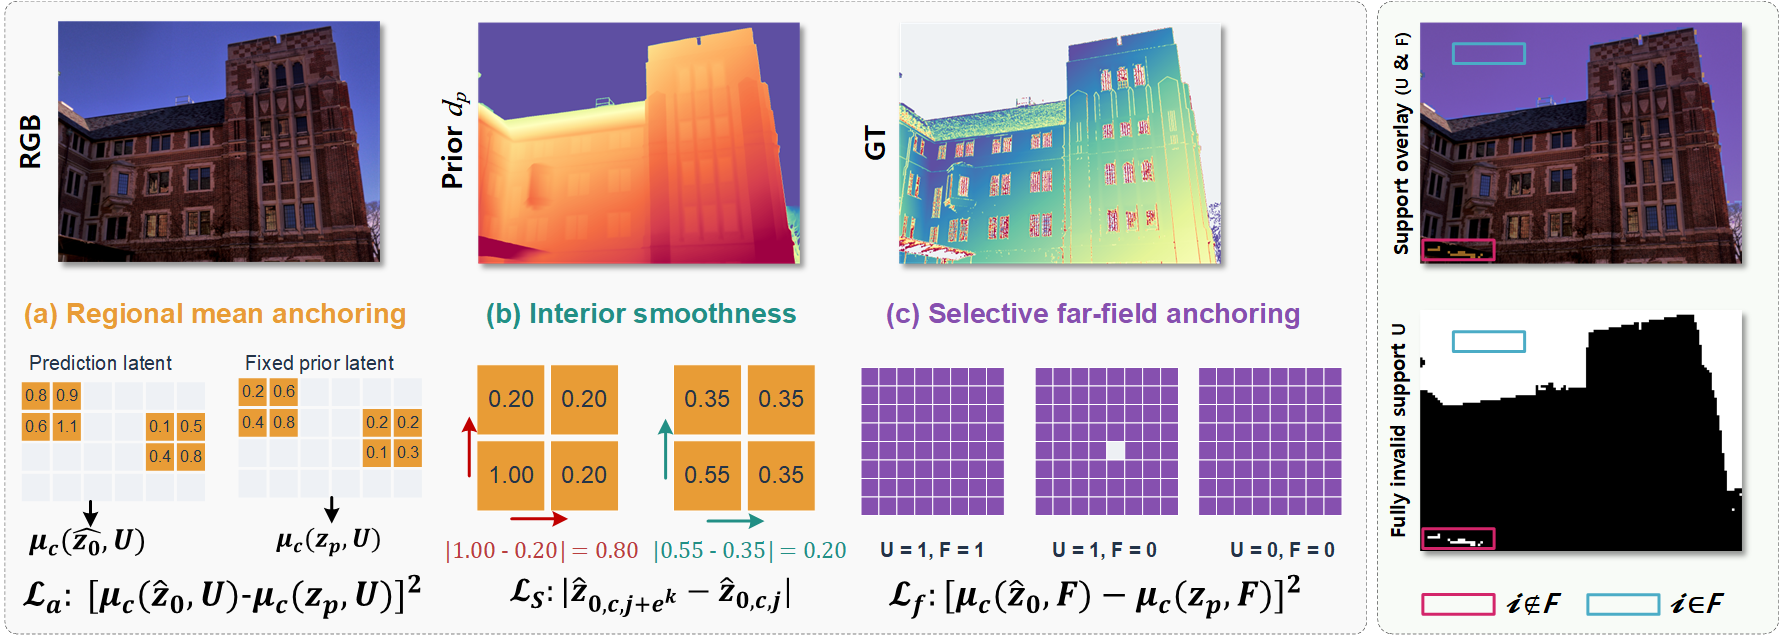
\includegraphics[width=\textwidth]{pdf/VGC.png}
	\caption{VGC illustrated on a DIODE outdoor example~\cite{vasiljevic2019diode}. Top: RGB, prior depth $d_p$, and GT depth. (a) Match channel-wise latent means over fully invalid support $U$. (b) Penalize horizontal and vertical differences between neighboring cells within $U$. (c) Apply an additional mean anchor over far-field subset $F$: a cell must belong to $U$ and all prior pixels in its $8\times8$ block must satisfy $d_p\geq0.5$. Right: support overlay and binary $U$ mask (white); cyan and magenta boxes mark examples inside and outside $F$. Numerical examples are schematic.}
	\label{fig:vgc}
\end{figure*}


\section{Method}
\label{sec:method}
\subsection{Overview}
\label{sec:overview}
Given an RGB image $X$, the goal is to predict an affine-invariant depth map $\hat d$. Figure~\ref{fig:framework} summarizes the framework. A frozen depth estimator supplies an auxiliary prior for conditional denoising and a weak reference for missing-depth regions. We first define the latent inputs in Sec.~\ref{sec:conditioning}, then introduce validity-guided completion in Sec.~\ref{sec:vgc}. Section~\ref{sec:diffusion} describes the diffusion training objective and noise construction, and Sec.~\ref{sec:inference} gives the multi-step inference procedure.

\subsection{Auxiliary Conditioning}
\label{sec:conditioning}
Training uses an RGB image $X\in[-1,1]^{3\times H\times W}$, a depth map $d$, and its binary validity mask $M$. We normalize $d$ using the 2nd and 98th percentiles of its valid positive depths, linearly map this interval to $[-1,1]$, and clip the result to obtain $\tilde d$. Let $\mathcal E$ denote the frozen VAE encoder, including its posterior-mean extraction and latent scaling factor of $0.18215$. The RGB and clean depth latents are $z_x=\mathcal E(X)$ and $z_d=\mathcal E(\operatorname{Rep}_3(\tilde d))$, where $\operatorname{Rep}_3$ copies a depth map into three channels. Each latent has $C=4$ channels and spatial size $h\times w$.

Following the prior-conditioned refinement pattern of BetterDepth~\cite{zhang2024betterdepth}, we use frozen Depth Anything V2-Giant~\cite{Li2024DepthV2} to obtain the auxiliary prior. Its RGB input is converted from $[-1,1]$ to $[0,1]$ and standardized with ImageNet mean and standard deviation. Its raw relative disparity $p$ is mapped to
\begin{equation}
	d_p=1-2\operatorname{clip}_{[0,1]}
	\left(\frac{p-q_2(p)}{\max(q_{98}(p)-q_2(p),\epsilon)}\right),
	\label{eq:prior_norm}
\end{equation}
where $q_2$ and $q_{98}$ are computed over all pixels of each prior image, and $\epsilon=10^{-6}$. This gives $d_p$ the same input range and near/far convention as $\tilde d$: $-1$ denotes near and $+1$ far. The prior remains relative depth.

The prior latent $z_p=\mathcal E(\operatorname{Rep}_3(d_p))$ is concatenated with $z_x$ and the noisy depth latent $z_t$ at timestep $t$:
\begin{equation}
	c_t=\operatorname{Cat}[z_x,z_p,z_t]\in\mathbb R^{12\times h\times w}.
	\label{eq:conditioning}
\end{equation}
The pretrained four-channel input convolution is expanded to twelve channels by repeating its weights three times and dividing them by three, with its bias retained. Only U-Net weights are optimized; the VAE, text encoder, and auxiliary estimator remain frozen, and the text condition is an empty-prompt embedding. The prior is computed before denoising and serves both as a conditioning input during training and inference and as a detached reference for VGC during training.

% 完全无效 latent 单元占比至少 8% 时启用 VGC。
\subsection{Validity-Guided Completion}
\label{sec:vgc}
\subsubsection{Conservative support}
We derive the loss supports from the GT validity mask $M$. Let $B_j$ be the $8\times8$ image block associated with latent cell $j$. We form distinct masks
\begin{equation}
	V_j=\prod_{i\in B_j}M_i,\qquad
	U_j=\prod_{i\in B_j}(1-M_i).
	\label{eq:support}
\end{equation}
Figure~\ref{fig:uv_shown} contrasts fully valid cells ($V$), fully invalid cells ($U$), and mixed cells, which belong to neither set; thus $U\ne1-V$ in general. Masks are broadcast over latent channels. Mixed cells are excluded from direct loss support, although the VAE receptive field and shared U-Net parameters can still couple neighboring regions.

\begin{figure}[!t]
	\centering
	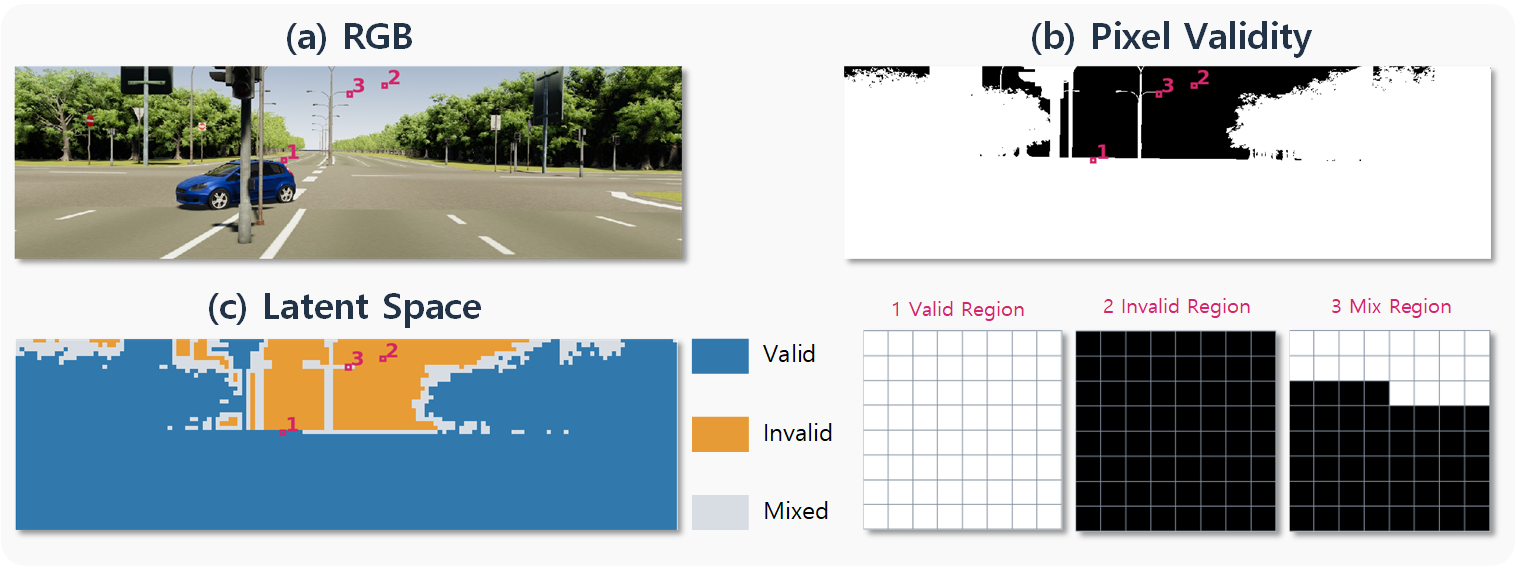
\includegraphics[width=\linewidth]{pdf/UV_SHOWN.png}
	\caption{Conservative latent supports in a Virtual KITTI 2 example~\cite{cabon2020virtual}. (a) RGB. (b) Pixel validity $M$ (white: valid; black: invalid). (c) Fully valid cells $V$ (blue), fully invalid cells $U$ (orange), and mixed cells (gray). Enlarged $8\times8$ blocks illustrate the three cases; mixed blocks belong to neither $U$ nor $V$.}
	\label{fig:uv_shown}
\end{figure}

For each sample $b$, completion is activated when fully invalid latent cells occupy at least a fraction $\rho=0.08$ of its entire $h\times w$ latent grid:
\begin{equation}
	g_b=\mathbf1\!\left[\frac{1}{hw}\sum_j U_{bj}\geq\rho\right].
	\label{eq:gate}
\end{equation}
This limits the influence of small missing-depth holes. It is not a semantic classifier; large invalid regions can include distant surfaces and indoor measurement failures as well as sky.
Figure~\ref{fig:vgc} illustrates the three completion constraints and their respective supports.

\subsubsection{Regional anchoring and interior smoothness}
Let $\hat z_0$ denote the clean depth latent reconstructed from the U-Net's velocity prediction at a sampled training timestep, as defined in Eq.~\eqref{eq:clean}. The VGC losses act directly on this reconstruction. For a spatial mask $A$, define the channel-wise regional mean
\begin{equation}
	\mu_{bc}(z,A)=\frac{\sum_j A_{bj}z_{bcj}}
	{\max(\sum_j A_{bj},\epsilon)}.
	\label{eq:region_mean}
\end{equation}
Here $b$, $c$, and $j$ index samples, latent channels, and spatial cells, respectively. For each sample and channel, the mean pools all selected cells, including disconnected regions; no connected-component partition is used. The basic anchor matches means over invalid support:
\begin{equation}
	\mathcal L_a=
	\frac{\sum_{b,c}g_b[\mu_{bc}(\hat z_0,U)-\mu_{bc}(z_p,U)]^2}
	{C\max(\sum_b g_b,\epsilon)}.
	\label{eq:anchor}
\end{equation}
The anchor is averaged over eligible samples and channels. The teacher latent is detached, so its values provide a fixed reference while gradients pass through $\hat z_0$ to the U-Net. A channel-wise mean allows local predictions to differ from the teacher, and a latent channel value should not be interpreted directly as metric distance.

To penalize unsupported variations, let $A^U_k(b,j)=g_bU_{bj}U_{b,j+e_k}$ for horizontal and vertical neighbors $k\in\{x,y\}$. With masks broadcast over channels, we use
\begin{equation}
	\mathcal L_s=\frac12\sum_{k\in\{x,y\}}
	\frac{\sum_{b,c,j} A^U_k(b,j)|\nabla_k\hat z_{0,bcj}|}
	{\max(\sum_{b,c,j} A^U_k(b,j),\epsilon)}.
	\label{eq:smooth}
\end{equation}
Each direction is averaged over all eligible neighbor pairs across the batch and channels. Only pairs wholly inside eligible invalid regions contribute. This removes a direct smoothing penalty across the valid/invalid boundary; the VAE receptive field and shared U-Net parameters can still affect decoded boundaries.

\subsubsection{Selective far-field anchor}
The basic invalid-region mean may combine several causes of missing depth. We add a second anchor on cells for which all underlying prior pixels indicate far depth:
\begin{equation}
	F_j=U_j\prod_{i\in B_j}\mathbf1[d_{p,i}\geq\tau],\qquad\tau=0.5.
	\label{eq:far_mask}
\end{equation}
A sample must pass the invalid-region gate, and its selected far-field cells must occupy at least $\rho_f=0.02$ of the entire latent grid:
\begin{equation}
	h_b=g_b\mathbf1\!\left[\frac{1}{hw}\sum_j F_{bj}\geq\rho_f\right].
\end{equation}
We then compute
\begin{equation}
	\mathcal L_f=
	\frac{\sum_{b,c}h_b[\mu_{bc}(\hat z_0,F)-\mu_{bc}(z_p,F)]^2}
	{C\max(\sum_b h_b,\epsilon)}.
	\label{eq:far_anchor}
\end{equation}
The far-field fraction is measured against $hw$, not against the size of $U$. The threshold $\tau$ is applied to the normalized image-space prior $d_p$ in Eq.~\eqref{eq:prior_norm}; it is a relative-depth threshold, not a confidence score or a distance in meters. The additional mean constraint is intended to reduce near-depth drift within this subset while the basic anchor still covers all eligible invalid cells.

The complete completion objective is
\begin{equation}
	\mathcal L_{\mathrm{VGC}}=0.02\mathcal L_a+0.005\mathcal L_s+0.01\mathcal L_f.
	\label{eq:vgc}
\end{equation}
Empty eligible sets contribute zero. The low weights reflect the uncertainty of the teacher and of the invalid-region selection.

\subsection{Diffusion Training with an Aligned Endpoint}
\label{sec:diffusion}
\subsubsection{Velocity prediction and terminal SNR}
For each training image, we independently sample one timestep $t$ uniformly from $\{0,\ldots,T-1\}$ and form a noisy state from the clean depth latent $z_d$. Write $a_t=\sqrt{\bar\alpha_t}$ and $b_t=\sqrt{1-\bar\alpha_t}$. The forward process and velocity target are
\begin{equation}
	z_t=a_tz_d+b_t\epsilon_t,\qquad
	v_t=a_t\epsilon_t-b_tz_d.
	\label{eq:velocity}
\end{equation}
The U-Net predicts $\hat v_t=f_\theta(c_t,t)$, giving
\begin{equation}
	\hat z_0=a_tz_t-b_t\hat v_t.
	\label{eq:clean}
\end{equation}
Each training forward pass predicts velocity once at the sampled timestep. Gradient consistency and VGC are evaluated on the resulting $\hat z_0$, without unrolling a multi-step denoising trajectory or decoding a depth image.
We rescale the pretrained schedule so that $\bar\alpha_{T-1}=0$ and start inference at this final timestep, following terminal-SNR alignment~\cite{lin2024common}. Equation~\eqref{eq:clean} remains finite there, unlike reconstruction that divides by $a_t$.

\subsubsection{Endpoint-aware structured noise}
Away from the endpoint, we retain annealed multi-resolution noise, as used in Marigold training~\cite{Ke2025Marigold}, and add a channel-wise Gaussian offset. Define
\begin{equation}
	s_t=\operatorname{clip}_{[0,1]}
	\left(\frac{1-t/(T-1)}{0.10}\right),\qquad
	\lambda_t=0.9\frac{t}{T-1}s_t.
	\label{eq:fade}
\end{equation}
The multi-resolution construction sums a full-resolution Gaussian field and upsampled random fields with coefficients $\lambda_t^i$, beginning at $i=0$, then normalizes by the composite standard deviation. Up to ten levels are used, stopping when a spatial dimension reaches one; the implementation samples downscale factors between two and four. Its standard-deviation normalization is computed over the generated batch tensor. With an independent offset $\xi\sim\mathcal N(0,I)$ of shape $C\times1\times1$, broadcast spatially, the noise is
\begin{equation}
	\epsilon_t=\epsilon_{\mathrm{MR}}(\lambda_t)+0.1s_t\xi,
	\quad t<T-1.
	\label{eq:noise}
\end{equation}
At $t=T-1$, the implementation explicitly replaces the composite noise with a fresh standard Gaussian. This matters because the normalization and the zeroth multi-resolution term do not disappear merely by setting the strength to zero. The exact endpoint consequently matches pure-noise initialization. The augmentation provides low-frequency perturbations during training without retaining an offset at the terminal timestep.

\subsubsection{Valid-region objectives}
For $\operatorname{SNR}(t)=\bar\alpha_t/(1-\bar\alpha_t)$, our velocity-space weight is
\begin{equation}
	w_v(t)=\frac{\min\{\max[\operatorname{SNR}(t),\eta],\gamma\}}
	{\operatorname{SNR}(t)+1},\quad \eta=0.05,\ \gamma=5.
	\label{eq:snr}
\end{equation}
This adopts Min-SNR weighting~\cite{hang2023efficient} with a small lower floor, so the pure-noise endpoint has a nonzero weight. The primary objective is evaluated in velocity space:
\begin{equation}
	\mathcal L_v=
	\frac{\sum_{b,c,j} V_{bj}w_v(t_b)(\hat v_{bcj}-v_{bcj})^2}
	{\max(\sum_{b,c,j}V_{bj},1)}.
	\label{eq:valid_loss}
\end{equation}
It is not an unweighted clean-latent reconstruction loss, and its numerical scale should not be compared directly with losses from another parameterization.

For adjacent pairs with two valid endpoints, $A^V_k(b,j)=V_{bj}V_{b,j+e_k}$, latent gradient consistency is
\begin{equation}
	\mathcal L_g=\sum_{k\in\{x,y\}}
	\frac{\sum_{b,c,j}A^V_k(b,j)
		\big||\nabla_k\hat z_{0,bcj}|-|\nabla_k z_{d,bcj}|\big|}
	{\max(\sum_{b,c,j}A^V_k(b,j),1)}.
	\label{eq:grad}
\end{equation}
This matches gradient magnitudes rather than signed gradients. In contrast to invalid-region smoothness, it preserves the magnitude of GT latent variations on fully valid neighbor pairs. The total loss is
\begin{equation}
	\mathcal L=\mathcal L_v+0.1\mathcal L_g+\mathcal L_{\mathrm{VGC}}.
	\label{eq:total}
\end{equation}
VGC and gradient consistency are not multiplied by $w_v(t)$ and have no additional timestep gate. Valid supervision learns geometry where GT is available, while completion provides limited guidance where that supervision is missing.

\subsection{Multi-Step Inference}
\label{sec:inference}
At inference, we compute $z_x$ and $z_p$ from the input image, initialize $z_{T-1}\sim\mathcal N(0,I)$, and apply 50 DDIM steps~\cite{song2020denoising} using the saved training-compatible scheduler with trailing timestep spacing. Each step concatenates the fixed conditions $z_x,z_p$ with the current noisy depth latent, predicts velocity, and updates that latent through the DDIM scheduler. Unlike the single sampled-timestep forward pass used for training, inference follows the complete selected denoising trajectory. The final latent is divided by $0.18215$ and decoded with the frozen VAE, its three output channels are averaged, and the result is clipped to $[-1,1]$ and mapped to $[0,1]$, with larger values denoting farther depth. No training loss, ground truth, or validity mask is needed for inference; DA2 remains a conditioning input. The standard setting uses one prediction per image rather than an ensemble.

\section{Experiments}
\label{sec:experiments}
Our evaluation measures depth accuracy across five datasets and isolates component contributions on NYUv2 and KITTI. We additionally inspect sky behavior qualitatively on KITTI test images, since valid-depth metrics alone do not measure sky-depth collapse.

\subsection{Training Data and Implementation}
\label{sec:implementation}
The U-Net is initialized from Stable Diffusion 2.1 and trained on Hypersim~\cite{roberts2021hypersim} and Virtual KITTI 2~\cite{cabon2020virtual}. Training uses an NVIDIA RTX 6000 Ada Generation GPU, and evaluation uses an NVIDIA RTX 5090 GPU. Hypersim inputs are resized to $480\times640$, and Virtual KITTI inputs use the KITTI benchmark crop. Virtual KITTI training validity is restricted to depths between zero and 80\,m. Values outside this interval are excluded from valid-depth supervision; this exclusion is not a semantic sky annotation.

Training uses Adam, an effective batch size of 42, and 23,000 optimizer updates. A microbatch size of seven is accumulated over six iterations. The initial learning rate is $3\times10^{-5}$, with 100 warm-up steps and an exponential schedule configured to reach a factor of 0.01 at update 25,000; training stops at 23,000 without shortening that schedule. Horizontal flipping has probability 0.5. The training and data-loader seeds are both 2024. The VAE, text encoder, and DA2-Giant remain frozen. All loss weights and gating thresholds are specified in Sec.~\ref{sec:method} and are held fixed across datasets.

We use progressive dataset sampling to increase outdoor exposure while retaining Hypersim as the majority source. Each microbatch is drawn from one dataset. The Virtual KITTI probability remains at 0.1 for the first 20\% of training, increases linearly to 0.2 over the next 60\%, and stays at 0.2 for the final 20\%; the Hypersim probability is its complement. The transition spans optimizer updates 4,600--18,400. Progress is measured in optimizer updates, independently of the sampled diffusion timestep, and resumes from the saved training position.

Each component ablation starts independently from the same base model and uses the same budget and progressive sampling protocol. We evaluate the final checkpoint rather than selecting a checkpoint on a test set. Inference uses 50 DDIM steps, ensemble size one, seed 2024, and native input resolution unless a dataset-specific preprocessing rule is explicitly stated. Evaluation must load the scheduler saved beside its U-Net; mixing schedules would confound the terminal-alignment comparison.

\subsection{Evaluation Protocol}
\label{sec:protocol}
NYUv2~\cite{silberman2012indoor} and KITTI~\cite{geiger2013vision} are the primary controlled evaluation datasets. We use the repository's NYUv2 labeled test list with its Eigen validity mask, and the KITTI Eigen test list with benchmark cropping and the Eigen evaluation mask. Predictions are aligned to metric ground truth by a per-image least-squares scale and shift fit over valid pixels, then clipped to the dataset evaluation range (10\,m for NYUv2 and 80\,m for KITTI). The fit is an evaluation operation, not metric calibration available at deployment.

For valid pixels $\Omega$ and aligned positive predictions $d_i^*$, the two reported metrics are
\begin{equation}
	\operatorname{AbsRel}=\frac{1}{|\Omega|}
	\sum_{i\in\Omega}\frac{|d_i^*-d_i|}{d_i},
\end{equation}
\begin{equation}
	\delta_1=\frac{1}{|\Omega|}\sum_{i\in\Omega}
	\mathbf1\!\left[\max\left(\frac{d_i^*}{d_i},\frac{d_i}{d_i^*}\right)<1.25\right].
\end{equation}
Tables display $100\times\operatorname{AbsRel}$ and $100\times\delta_1$. Lower AbsRel and higher $\delta_1$ are better. All paired ablations use identical test images, masks, alignment, and inference settings. The main comparison additionally evaluates the complete model on ETH3D~\cite{schops2017multi}, ScanNet~\cite{dai2017scannet}, and DIODE~\cite{vasiljevic2019diode}, using their available valid-depth masks and evaluation ranges. Component ablations are restricted to NYUv2 and KITTI.

\subsection{Main Benchmark Comparison}
\label{sec:main_results}
Table~\ref{tab:main} places ApDepth-G alongside discriminative and generative depth estimators. The comparison is intended to test whether improved sky behavior is accompanied by competitive indoor and outdoor depth accuracy. Its training-data column describes task-adaptation data as supplied, not all data used to pretrain either the diffusion backbone or the auxiliary teacher. In particular, using DA2 introduces external learned information that must be acknowledged when comparing supervision budgets.

\draftnote{Published baseline rows in Table~\ref{tab:main} follow the comparison reported by Marigold V2~\cite{pavlovic2026marigoldv2}. The ApDepth and ApDepth-G rows are author-supplied records, not yet verified measurements of the current checkpoint. Final interpretation of those two rows and cross-method protocol verification remain pending.}
% Baseline values are transcribed from the cited papers; author rows remain provisional.
\begin{table*}[!t]
	\centering
	\caption{Zero-shot affine-invariant depth comparison. AbsRel is multiplied by 100 and $\delta_1$ is in percent. Baselines are transcribed from Marigold V2~\cite{pavlovic2026marigoldv2}; an em dash denotes an unavailable record. Training counts refer to task-specific samples and exclude backbone or generative-model pretraining. The ApDepth and ApDepth-G records are author-supplied and remain provisional; no best/second-best styling is applied.}
	\label{tab:main}
	\setlength{\tabcolsep}{4pt}
	\footnotesize
	\begin{tabular}{@{}llrrrrrrrrrrr@{}}
		\toprule
		Type           & Method                                      & Training & \multicolumn{2}{c}{NYUv2} & \multicolumn{2}{c}{KITTI} & \multicolumn{2}{c}{ETH3D} & \multicolumn{2}{c}{ScanNet} & \multicolumn{2}{c}{DIODE} \\
		\cmidrule(lr){4-5}\cmidrule(lr){6-7}\cmidrule(lr){8-9}\cmidrule(lr){10-11}\cmidrule(l){12-13}
		               &                                             & data     & AbsRel$\downarrow$ & $\delta_1\uparrow$ & AbsRel$\downarrow$ & $\delta_1\uparrow$ & AbsRel$\downarrow$ & $\delta_1\uparrow$ & AbsRel$\downarrow$ & $\delta_1\uparrow$ & AbsRel$\downarrow$ & $\delta_1\uparrow$ \\
		\midrule
		Discriminative & MiDaS~\cite{ranftl2020towards}              & 2M       & 11.1 & 88.5 & 23.6 & 63.0 & 18.4 & 75.2 & 12.1 & 84.6 & \textemdash & \textemdash \\
		               & DPT~\cite{ranftl2021vision}                 & 1.4M     & 9.8 & 90.3 & 10.0 & 90.1 & 7.8 & 94.6 & 8.2 & 93.4 & \textemdash & \textemdash \\
		               & Depth Anything V2~\cite{Li2024DepthV2}      & 63.5M    & 4.3 & 98.0 & 8.0 & 94.6 & 6.2 & 98.0 & 4.3 & 98.1 & 6.6 & 95.2 \\
		\midrule
		Generative     & Marigold~\cite{ke2024repurposing}          & 74K      & 5.5 & 96.4 & 9.9 & 91.6 & 6.5 & 96.0 & 6.4 & 95.1 & 10.0 & 90.7 \\
		               & GeoWizard~\cite{fu2025geowizard}           & 280K     & 5.2 & 96.6 & 9.7 & 92.1 & 6.4 & 96.1 & 6.1 & 95.3 & 12.0 & 89.8 \\
		               & DepthFM~\cite{gui2024depthfm}              & 74K      & 6.0 & 95.5 & 9.1 & 90.2 & 6.5 & 95.4 & 6.6 & 94.9 & \textemdash & \textemdash \\
		               & GenPercept~\cite{xu2024genpercept}         & 90K      & 5.6 & 96.0 & 9.9 & 90.4 & 6.2 & 95.8 & 5.6 & 96.5 & \textemdash & \textemdash \\
		               & Lotus~\cite{he2025lotus}                   & 59K      & 5.4 & 96.8 & 8.5 & 92.2 & 5.9 & 97.0 & 5.9 & 95.7 & 9.8 & 92.4 \\
		               & Lotus-2~\cite{he2025lotus2}                & 59K      & 3.7 & 97.6 & 6.7 & 94.1 & 4.1 & 98.6 & 4.0 & 97.2 & 6.5 & 95.5 \\
		               & PPD (512)~\cite{xu2025pixel}               & 54K      & 4.3 & 97.4 & 8.0 & 93.1 & 4.5 & 97.7 & 4.5 & 97.3 & 7.0 & 95.5 \\
		               & PPD (1024)~\cite{xu2025pixel}              & 125K     & 4.1 & 97.7 & 7.0 & 95.5 & 4.3 & 98.0 & 4.6 & 97.2 & 6.8 & 95.9 \\
		               & InfiniDepth~\cite{yu2026infinidepth}       & 3.1M     & 4.3 & 97.6 & 8.7 & 92.3 & 6.1 & 95.4 & 4.7 & 96.9 & 6.4 & 95.8 \\
		               & DepthMaster~\cite{song2026depthmaster}     & 74K      & 4.8 & 97.0 & 9.1 & 91.1 & 5.4 & 97.4 & 5.8 & 95.6 & 8.0 & 94.3 \\
		               & FE2E~\cite{wang2026fe2e}                   & 71K      & 3.8 & 97.6 & 6.5 & 96.0 & 3.8 & 98.7 & 4.3 & 97.1 & 5.6 & 96.4 \\
		               & Marigold V2~\cite{pavlovic2026marigoldv2} & 74K      & 3.6 & 98.0 & 5.4 & 97.4 & 2.8 & 99.2 & 3.7 & 97.9 & 5.2 & 97.1 \\
		\midrule
		               & ApDepth (Ours)~\cite{wang2026apdepth}      & 74K      & 4.5 & 97.3 & 8.7 & 93.7 & 5.6 & 96.3 & 4.5 & 97.3 & 8.3 & 93.2 \\
		               & ApDepth-G (Ours)                           & 74K      & 4.5 & 97.2 & 8.0 & 94.4 & 5.1 & 96.9 & 4.5 & 97.3 & 7.8 & 94.2 \\
		\bottomrule
	\end{tabular}
\end{table*}


% RESULT TEXT: add interpretation only after replacing/confirming the records.
% Positive hypothesis to test: VGC improves sky stability while retaining
% competitive NYUv2/KITTI accuracy. Do not present this as a measured finding yet.

\subsection{Controlled Ablations}
\label{sec:ablations}
Tables~\ref{tab:sky_ablation} and~\ref{tab:training_ablation} cover the eleven configurations in \texttt{config/ablation}. The complete method is the shared reference. Unless stated otherwise, each row changes only the named component. Every run retains corrected DA2 preprocessing and output ordering, velocity prediction, the frozen original decoder, progressive dataset sampling, and the same training budget. The value \texttt{TBD} denotes an experiment awaiting measurement, not zero or a missing baseline score.

\subsubsection{Completion and far-field supervision}
Removing $\mathcal L_a$, $\mathcal L_s$, or $\mathcal L_f$ individually measures each constraint's contribution with the other two retained. Removing all of VGC keeps prior conditioning but eliminates all three constraints. These comparisons assess regional anchoring, interior smoothness, and selective far-field guidance through NYUv2/KITTI metrics and qualitative sky comparisons on KITTI.

\subsubsection{Terminal alignment}
The terminal-SNR ablation disables zero-terminal-SNR rescaling, uses leading rather than trailing inference timesteps, sets the Min-SNR floor to zero, and disables terminal noise fading and Gaussian replacement. It retains velocity prediction. This is a grouped ablation of a coordinated training/inference design; it does not attribute any measured effect to one of its four changes alone.

\subsubsection{Auxiliary prior dependence}
The no-DA2-information row sets the four prior-conditioning channels to zero and disables VGC, while retaining the twelve-channel U-Net. It measures the contribution of all teacher information rather than a single loss. Comparing it with the no-VGC row isolates prior conditioning with completion disabled in both. The same channels are zeroed during inference. This control is not an eight-channel architecture comparison, nor a timing measurement of an optimized teacher-free deployment. The ordinary complete model continues to use DA2 at inference.

\begin{table}[!t]
	\centering
	\caption{Core ablations on NYUv2 and KITTI. All entries await measurement. IDs match the configuration filenames. AbsRel is multiplied by 100; $\delta_1$ is in percent.}
	\label{tab:sky_ablation}
	\setlength{\tabcolsep}{3pt}
	\footnotesize
	\begin{tabular}{@{}llrrrr@{}}
		\toprule
		   &                        & \multicolumn{2}{c}{NYUv2} & \multicolumn{2}{c}{KITTI}                                           \\
		\cmidrule(lr){3-4}\cmidrule(l){5-6}
		ID & Configuration          & AbsRel$\downarrow$        & $\delta_1\uparrow$        & AbsRel$\downarrow$ & $\delta_1\uparrow$ \\
		\midrule
		00 & Full                   & \pending                  & \pending                  & \pending           & \pending           \\
		01 & w/o far anchor         & \pending                  & \pending                  & \pending           & \pending           \\
		02 & w/o VGC                & \pending                  & \pending                  & \pending           & \pending           \\
		09 & w/o regional anchor    & \pending                  & \pending                  & \pending           & \pending           \\
		10 & w/o interior smoothness & \pending                 & \pending                  & \pending           & \pending           \\
		03 & w/o terminal alignment & \pending                  & \pending                  & \pending           & \pending           \\
		08 & w/o DA2 information    & \pending                  & \pending                  & \pending           & \pending           \\
		\bottomrule
	\end{tabular}
\end{table}


\subsubsection{Supporting optimization components}
The remaining controls remove Min-SNR weighting, multi-resolution noise, channel offset noise, or latent gradient consistency individually. Disabling Min-SNR means an unweighted velocity error, not setting its clipping parameter to zero. It also removes the floor's effect on that weighting. Disabling multi-resolution noise retains offset noise and endpoint alignment; disabling offset noise leaves the multi-resolution construction intact. These controls assess the support provided by established optimization techniques rather than present each technique as a new contribution.

\begin{table}[!t]
	\centering
	\caption{Supporting training components, with the same full-model reference as Table~\ref{tab:sky_ablation}. Values remain to be measured.}
	\label{tab:training_ablation}
	\setlength{\tabcolsep}{3pt}
	\footnotesize
	\begin{tabular}{@{}llrrrr@{}}
		\toprule
		   &                      & \multicolumn{2}{c}{NYUv2} & \multicolumn{2}{c}{KITTI}                                           \\
		\cmidrule(lr){3-4}\cmidrule(l){5-6}
		ID & Configuration        & AbsRel$\downarrow$        & $\delta_1\uparrow$        & AbsRel$\downarrow$ & $\delta_1\uparrow$ \\
		\midrule
		00 & Full                 & \pending                  & \pending                  & \pending           & \pending           \\
		04 & w/o Min-SNR          & \pending                  & \pending                  & \pending           & \pending           \\
		05 & w/o multi-res. noise & \pending                  & \pending                  & \pending           & \pending           \\
		06 & w/o offset noise     & \pending                  & \pending                  & \pending           & \pending           \\
		07 & w/o latent gradient  & \pending                  & \pending                  & \pending           & \pending           \\
		\bottomrule
	\end{tabular}
\end{table}


Loss magnitudes across these rows are not directly comparable because the objective changes. We compare held-out predictions and, for the most consequential comparisons, plan repeated training seeds to distinguish component effects from stochastic variation. No significance or error-bar claim is made from a single run.

\subsection{Qualitative Sky Analysis}
\label{sec:sky_eval}
Standard valid-depth benchmarks omit much of the sky, so KITTI AbsRel alone cannot establish that sky-depth collapse has been resolved. We therefore compare predictions on a fixed selection of KITTI test images containing sky, distant skylines, and vegetation boundaries. Panels show RGB, the complete model, the individual VGC ablations, the no-VGC model, and the auxiliary prior, with a shared near/far color convention and normalization rule. Enlarged skyline and sky-interior crops reveal discontinuities, spurious texture, and loss of distant structure. This analysis is qualitative; no sky-specific quantitative score is inferred from valid-depth metrics.

\section{Discussion and Limitations}
\label{sec:limitations}
The proposed completion is a weak constraint, not a proof of correct sky geometry. A foundation prior can itself be wrong, and an invalid region can contain a structured distant object rather than sky. Region means reduce pointwise imitation but can still transfer a biased regional response; smoothness can suppress legitimate distant structure. Conservative masks mitigate direct boundary penalties, while latent receptive fields and the shared denoiser prevent perfect spatial isolation.

The method also depends on the frozen prior at inference and retains the cost of 50 denoising steps. Its output is affine-invariant, so far-depth consistency does not imply calibrated metric infinity. Moreover, the interface correction to DA2 input normalization and depth ordering is a correctness fix that all comparisons must share; improvements caused by that correction cannot be attributed to VGC. Finally, the supplied benchmark records require checkpoint/protocol verification, while the controlled component results remain to be completed.

\section{Conclusion}
\label{sec:conclusion}
We presented ApDepth-G as a multi-step depth framework aimed at reducing sky-depth collapse through explicit treatment of missing supervision. The method combines conservative validity masks, weak regional completion, and selective far-field anchoring, supported by terminal-aligned diffusion training. A frozen auxiliary depth model provides conditioning and a weak reference, while the core design concerns how that information constrains otherwise under-supervised regions. The evaluation protocol combines five-dataset benchmarking, NYUv2/KITTI ablations, and qualitative sky comparisons. Quantitative conclusions will be completed after the controlled experiments.
\section*{Acknowledgment}
This work was supported by the National Natural Science Foundation of China (62073227) and the Liaoning Provincial Science and Technology Department Foundation (2023JH2/101300212).

\bibliographystyle{IEEEtran}
\bibliography{ieee-dc-template}
\end{document}


